\documentclass[a4paper]{article}
\usepackage[]{graphicx}\usepackage[]{color}
% maxwidth is the original width if it is less than linewidth
% otherwise use linewidth (to make sure the graphics do not exceed the margin)
\makeatletter
\def\maxwidth{ %
  \ifdim\Gin@nat@width>\linewidth
    \linewidth
  \else
    \Gin@nat@width
  \fi
}
\makeatother

\definecolor{fgcolor}{rgb}{0.345, 0.345, 0.345}
\newcommand{\hlnum}[1]{\textcolor[rgb]{0.686,0.059,0.569}{#1}}%
\newcommand{\hlstr}[1]{\textcolor[rgb]{0.192,0.494,0.8}{#1}}%
\newcommand{\hlcom}[1]{\textcolor[rgb]{0.678,0.584,0.686}{\textit{#1}}}%
\newcommand{\hlopt}[1]{\textcolor[rgb]{0,0,0}{#1}}%
\newcommand{\hlstd}[1]{\textcolor[rgb]{0.345,0.345,0.345}{#1}}%
\newcommand{\hlkwa}[1]{\textcolor[rgb]{0.161,0.373,0.58}{\textbf{#1}}}%
\newcommand{\hlkwb}[1]{\textcolor[rgb]{0.69,0.353,0.396}{#1}}%
\newcommand{\hlkwc}[1]{\textcolor[rgb]{0.333,0.667,0.333}{#1}}%
\newcommand{\hlkwd}[1]{\textcolor[rgb]{0.737,0.353,0.396}{\textbf{#1}}}%
\let\hlipl\hlkwb

\usepackage{framed}
\makeatletter
\newenvironment{kframe}{%
 \def\at@end@of@kframe{}%
 \ifinner\ifhmode%
  \def\at@end@of@kframe{\end{minipage}}%
  \begin{minipage}{\columnwidth}%
 \fi\fi%
 \def\FrameCommand##1{\hskip\@totalleftmargin \hskip-\fboxsep
 \colorbox{shadecolor}{##1}\hskip-\fboxsep
     % There is no \\@totalrightmargin, so:
     \hskip-\linewidth \hskip-\@totalleftmargin \hskip\columnwidth}%
 \MakeFramed {\advance\hsize-\width
   \@totalleftmargin\z@ \linewidth\hsize
   \@setminipage}}%
 {\par\unskip\endMakeFramed%
 \at@end@of@kframe}
\makeatother

\definecolor{shadecolor}{rgb}{.97, .97, .97}
\definecolor{messagecolor}{rgb}{0, 0, 0}
\definecolor{warningcolor}{rgb}{1, 0, 1}
\definecolor{errorcolor}{rgb}{1, 0, 0}
\newenvironment{knitrout}{}{} % an empty environment to be redefined in TeX

\usepackage{alltt}
\newcommand{\SweaveOpts}[1]{}  % do not interfere with LaTeX
\newcommand{\SweaveInput}[1]{} % because they are not real TeX commands
\newcommand{\Sexpr}[1]{}       % will only be parsed by R




\usepackage[utf8]{inputenc}
%\usepackage[ngerman]{babel}
\usepackage{a4wide,paralist}
\usepackage{amsmath, amssymb, xfrac, amsthm}
\usepackage{dsfont}
\usepackage[usenames,dvipsnames]{xcolor}
\usepackage{amsfonts}
\usepackage{graphicx}
\usepackage{caption}
\usepackage{subcaption}
\usepackage{framed}
\usepackage{multirow}
\usepackage{bytefield}
\usepackage{csquotes}
\usepackage[breakable, theorems, skins]{tcolorbox}
\usepackage{hyperref}
\usepackage{cancel}
\usepackage{bm}


\input{../../style/common}

\tcbset{enhanced}

\DeclareRobustCommand{\mybox}[2][gray!20]{%
	\iffalse
	\begin{tcolorbox}[   %% Adjust the following parameters at will.
		breakable,
		left=0pt,
		right=0pt,
		top=0pt,
		bottom=0pt,
		colback=#1,
		colframe=#1,
		width=\dimexpr\linewidth\relax,
		enlarge left by=0mm,
		boxsep=5pt,
		arc=0pt,outer arc=0pt,
		]
		#2
	\end{tcolorbox}
	\fi
}

\DeclareRobustCommand{\myboxshow}[2][gray!20]{%
%	\iffalse
	\begin{tcolorbox}[   %% Adjust the following parameters at will.
		breakable,
		left=0pt,
		right=0pt,
		top=0pt,
		bottom=0pt,
		colback=#1,
		colframe=#1,
		width=\dimexpr\linewidth\relax,
		enlarge left by=0mm,
		boxsep=5pt,
		arc=0pt,outer arc=0pt,
		]
		#2
	\end{tcolorbox}
%	\fi
}


%exercise numbering
\renewcommand{\theenumi}{(\alph{enumi})}
\renewcommand{\theenumii}{\roman{enumii}}
\renewcommand\labelenumi{\theenumi}


\font \sfbold=cmssbx10

\setlength{\oddsidemargin}{0cm} \setlength{\textwidth}{16cm}


\sloppy
\parindent0em
\parskip0.5em
\topmargin-2.3 cm
\textheight25cm
\textwidth17.5cm
\oddsidemargin-0.8cm
\pagestyle{empty}

\newcommand{\kopf}[1] {
\hrule
\vspace{.15cm}
\begin{minipage}{\textwidth}
%akwardly i had to put \" here to make it compile correctly
	{\sf\bf Introduction to Machine Learning \hfill Exercise sheet #1\\
	 \url{https://introduction-to-machine-learning.netlify.app/} \hfill WiSe 2020/2021}
\end{minipage}
\vspace{.05cm}
\hrule
\vspace{1cm}}

\newenvironment{allgemein}
	{\noindent}{\vspace{1cm}}

\newcounter{aufg}
\newenvironment{aufgabe}
	{\refstepcounter{aufg}\textbf{Exercise \arabic{aufg}:}\\ \noindent}
	{\vspace{0.5cm}}

\newcounter{loes}
\newenvironment{loesung}
	{\refstepcounter{loes}\textbf{Solution \arabic{loes}:}\\\noindent}
	{\bigskip}
	
\newenvironment{bonusaufgabe}
	{\refstepcounter{aufg}\textbf{Exercise \arabic{aufg}*\footnote{This
	is a bonus exercise.}:}\\ \noindent}
	{\vspace{0.5cm}}

\newenvironment{bonusloesung}
	{\refstepcounter{loes}\textbf{Solution \arabic{loes}*:}\\\noindent}
	{\bigskip}



\begin{document}
% !Rnw weave = knitr



\input{../../latex-math/basic-math.tex}
\input{../../latex-math/basic-ml.tex}
\input{../../latex-math/ml-trees.tex}

\kopf{8}

\loesung{

\begin{enumerate}
  \item[a)]
  The spam data is a binary classification task where the aim is to classify an email as spam or no-spam.

\begin{knitrout}
\definecolor{shadecolor}{rgb}{0.969, 0.969, 0.969}\color{fgcolor}\begin{kframe}
\begin{alltt}
\hlkwd{library}\hlstd{(mlr3)}
\hlkwd{library}\hlstd{(mlr3learners)}
\hlkwd{library}\hlstd{(mlr3filters)}

\hlkwd{tsk}\hlstd{(}\hlstr{"spam"}\hlstd{)}
\end{alltt}
\begin{verbatim}
## <TaskClassif:spam> (4601 x 58)
## * Target: type
## * Properties: twoclass
## * Features (57):
##   - dbl (57): address, addresses, all, business, capitalAve,
##     capitalLong, capitalTotal, charDollar, charExclamation, charHash,
##     charRoundbracket, charSemicolon, charSquarebracket, conference,
##     credit, cs, data, direct, edu, email, font, free, george, hp, hpl,
##     internet, lab, labs, mail, make, meeting, money, num000, num1999,
##     num3d, num415, num650, num85, num857, order, original, our, over,
##     parts, people, pm, project, re, receive, remove, report, table,
##     technology, telnet, will, you, your
\end{verbatim}
\end{kframe}
\end{knitrout}
  \item[b)]

\begin{knitrout}
\definecolor{shadecolor}{rgb}{0.969, 0.969, 0.969}\color{fgcolor}\begin{kframe}
\begin{alltt}
\hlkwd{library}\hlstd{(rpart.plot)}
\end{alltt}


{\ttfamily\noindent\itshape\color{messagecolor}{\#\# Loading required package: rpart}}\begin{alltt}
\hlstd{task_spam} \hlkwb{<-} \hlkwd{tsk}\hlstd{(}\hlstr{"spam"}\hlstd{)}

\hlstd{learner} \hlkwb{<-} \hlkwd{lrn}\hlstd{(}\hlstr{"classif.rpart"}\hlstd{)}
\hlstd{learner}\hlopt{$}\hlkwd{train}\hlstd{(task_spam)}

\hlkwd{rpart.plot}\hlstd{(learner}\hlopt{$}\hlstd{model,} \hlkwc{roundint}\hlstd{=}\hlnum{FALSE}\hlstd{)}
\end{alltt}
\end{kframe}
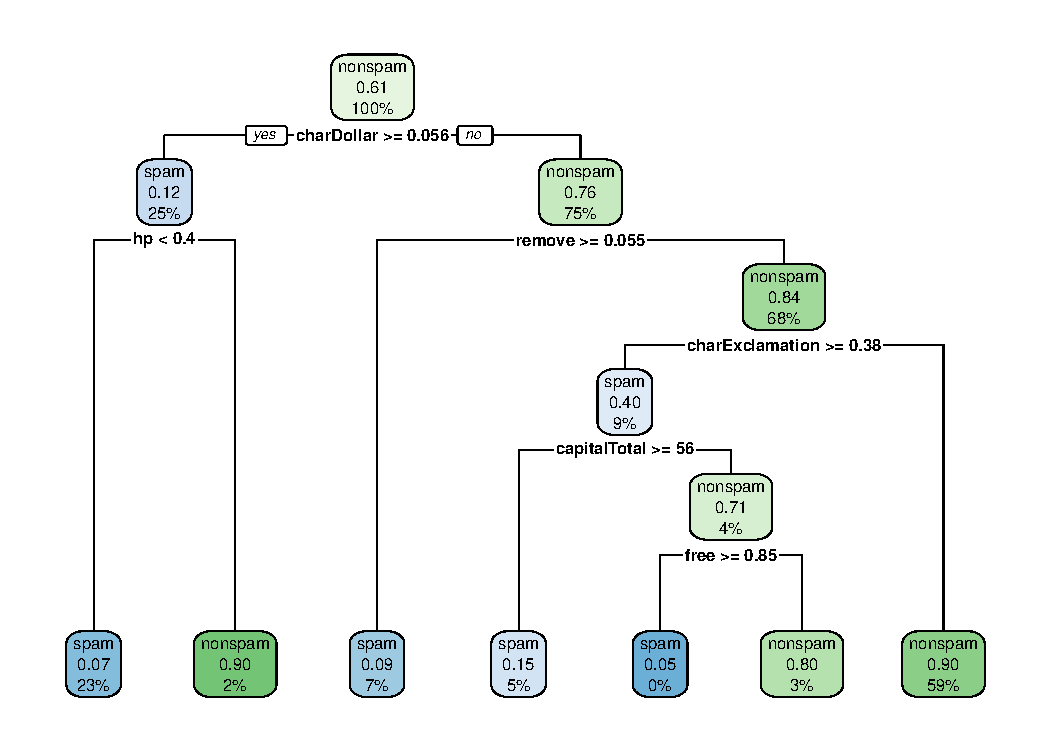
\includegraphics[width=\maxwidth]{figure/unnamed-chunk-3-1} 
\begin{kframe}\begin{alltt}
\hlkwd{set.seed}\hlstd{(}\hlnum{42}\hlstd{)}

\hlstd{subset1} \hlkwb{<-} \hlkwd{sample.int}\hlstd{(task_spam}\hlopt{$}\hlstd{nrow,} \hlkwc{size} \hlstd{=} \hlnum{0.8} \hlopt{*} \hlstd{task_spam}\hlopt{$}\hlstd{nrow)}
\hlstd{subset2} \hlkwb{<-} \hlkwd{sample.int}\hlstd{(task_spam}\hlopt{$}\hlstd{nrow,} \hlkwc{size} \hlstd{=} \hlnum{0.8} \hlopt{*} \hlstd{task_spam}\hlopt{$}\hlstd{nrow)}

\hlstd{learner}\hlopt{$}\hlkwd{train}\hlstd{(task_spam,} \hlkwc{row_ids} \hlstd{= subset1)}
\hlkwd{rpart.plot}\hlstd{(learner}\hlopt{$}\hlstd{model,} \hlkwc{roundint}\hlstd{=}\hlnum{FALSE}\hlstd{)}
\end{alltt}
\end{kframe}
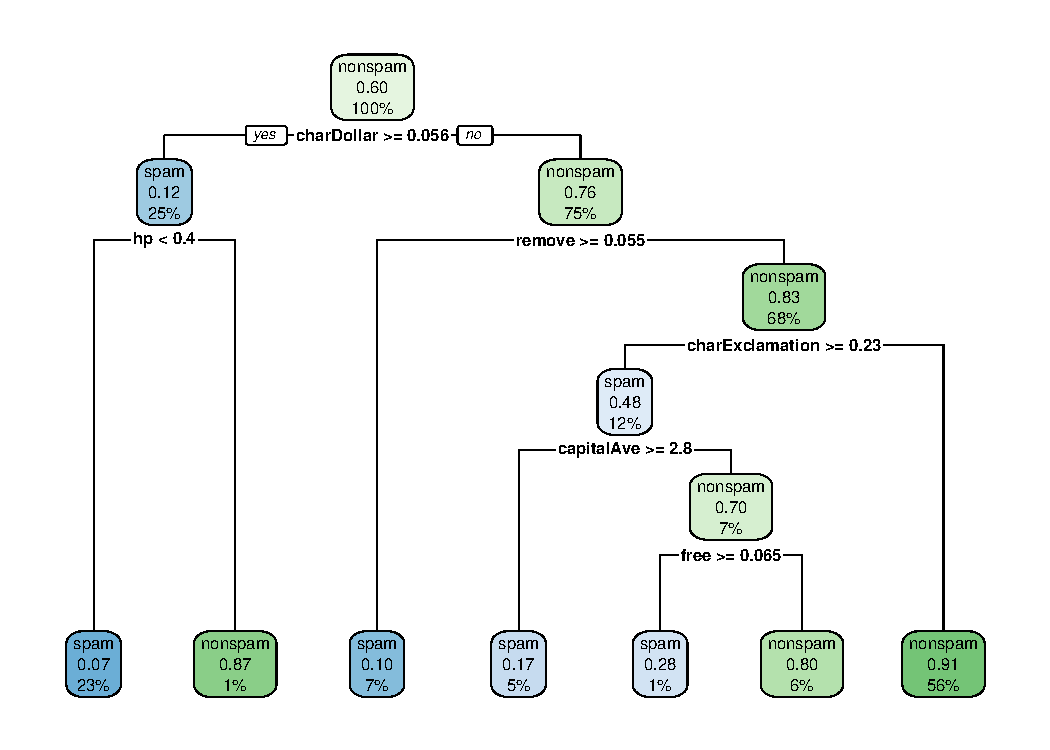
\includegraphics[width=\maxwidth]{figure/unnamed-chunk-3-2} 
\begin{kframe}\begin{alltt}
\hlstd{learner}\hlopt{$}\hlkwd{train}\hlstd{(task_spam,} \hlkwc{row_ids} \hlstd{= subset2)}
\hlkwd{rpart.plot}\hlstd{(learner}\hlopt{$}\hlstd{model,} \hlkwc{roundint}\hlstd{=}\hlnum{FALSE}\hlstd{)}
\end{alltt}
\end{kframe}
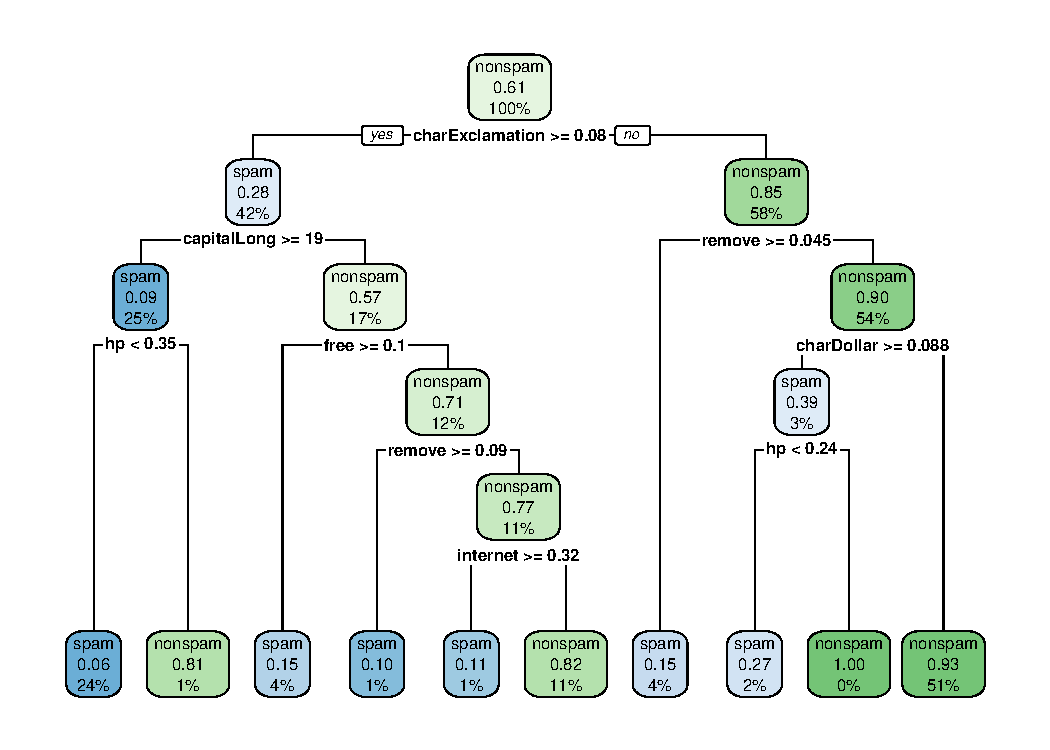
\includegraphics[width=\maxwidth]{figure/unnamed-chunk-3-3} 
\end{knitrout}
  Observation: Trees with different sample find different split points and variables, leading to different trees!

  \item[c)]

\begin{knitrout}
\definecolor{shadecolor}{rgb}{0.969, 0.969, 0.969}\color{fgcolor}\begin{kframe}
\begin{alltt}
\hlstd{learner} \hlkwb{<-} \hlkwd{lrn}\hlstd{(}\hlstr{"classif.ranger"}\hlstd{,} \hlstr{"oob.error"} \hlstd{=} \hlnum{TRUE}\hlstd{)}
\hlstd{learner}\hlopt{$}\hlkwd{train}\hlstd{(}\hlkwd{tsk}\hlstd{(}\hlstr{"spam"}\hlstd{))}

\hlstd{model} \hlkwb{<-} \hlstd{learner}\hlopt{$}\hlstd{model}

\hlstd{model}\hlopt{$}\hlstd{prediction.error}
\end{alltt}
\begin{verbatim}
## [1] 0.04542491
\end{verbatim}
\end{kframe}
\end{knitrout}

  \item[d)]

Variable importance in general measures the contributions of features to a model.
One way of computing the variable importance of the j-th variable is based on permutations of the OOB observations of the j-th variable, which measures the mean deacrease of the predictive accuracy induced by this permutation. To determine the $n$ variables with the biggest influence on the prediction quality, one can choose the $n$ variables with the highest variable importance based on permutations of the OOB,
e.g. for $n=5$:

\begin{knitrout}
\definecolor{shadecolor}{rgb}{0.969, 0.969, 0.969}\color{fgcolor}\begin{kframe}
\begin{alltt}
\hlstd{learner} \hlkwb{<-} \hlkwd{lrn}\hlstd{(}\hlstr{"classif.ranger"}\hlstd{,} \hlkwc{importance} \hlstd{=} \hlstr{"permutation"}\hlstd{,} \hlstr{"oob.error"} \hlstd{=} \hlnum{TRUE}\hlstd{)}
\hlstd{filter} \hlkwb{<-} \hlkwd{flt}\hlstd{(}\hlstr{"importance"}\hlstd{,} \hlkwc{learner} \hlstd{= learner)}
\hlstd{filter}\hlopt{$}\hlkwd{calculate}\hlstd{(}\hlkwd{tsk}\hlstd{(}\hlstr{"spam"}\hlstd{))}
\hlkwd{head}\hlstd{(}\hlkwd{as.data.table}\hlstd{(filter),} \hlnum{5}\hlstd{)}
\end{alltt}
\begin{verbatim}
##            feature      score
## 1:     capitalLong 0.04644338
## 2:              hp 0.04125252
## 3: charExclamation 0.03977957
## 4:          remove 0.03827180
## 5:      capitalAve 0.03424298
\end{verbatim}
\end{kframe}
\end{knitrout}

\end{enumerate}
}

\dlz


\loesung{
See \href{https://github.com/compstat-lmu/lecture_i2ml/blob/master/exercises/forests/ex_rnw/sol_dec_boundaries.R}{R code}
}

\dlz


\end{document}
